% !TEX encoding = UTF-8 Unicode
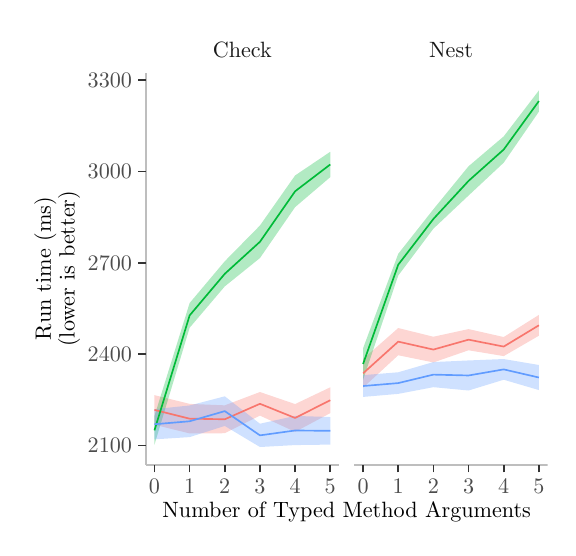
\begin{tikzpicture}[x=1pt,y=1pt]
\definecolor{fillColor}{RGB}{255,255,255}
\path[use as bounding box,fill=fillColor,fill opacity=0.00] (0,0) rectangle (187.90,180.67);
\begin{scope}
\path[clip] ( 42.64, 22.70) rectangle (112.52,164.42);
\definecolor{fillColor}{RGB}{248,118,109}

\path[fill=fillColor,fill opacity=0.30] ( 45.81, 47.89) --
	( 58.52, 44.72) --
	( 71.22, 44.20) --
	( 83.93, 49.01) --
	( 96.64, 44.66) --
	(109.34, 50.72) --
	(109.34, 41.38) --
	( 96.64, 34.62) --
	( 83.93, 40.50) --
	( 71.22, 34.12) --
	( 58.52, 34.04) --
	( 45.81, 37.20) --
	cycle;
\definecolor{fillColor}{RGB}{0,186,56}

\path[fill=fillColor,fill opacity=0.30] ( 45.81, 40.33) --
	( 58.52, 81.16) --
	( 71.22, 96.26) --
	( 83.93,109.18) --
	( 96.64,127.27) --
	(109.34,135.82) --
	(109.34,126.66) --
	( 96.64,115.83) --
	( 83.93, 97.42) --
	( 71.22, 87.18) --
	( 58.52, 72.23) --
	( 45.81, 29.98) --
	cycle;
\definecolor{fillColor}{RGB}{97,156,255}

\path[fill=fillColor,fill opacity=0.30] ( 45.81, 42.82) --
	( 58.52, 44.15) --
	( 71.22, 47.46) --
	( 83.93, 37.56) --
	( 96.64, 40.37) --
	(109.34, 39.98) --
	(109.34, 30.01) --
	( 96.64, 29.84) --
	( 83.93, 29.14) --
	( 71.22, 36.76) --
	( 58.52, 32.72) --
	( 45.81, 31.91) --
	cycle;
\definecolor{drawColor}{RGB}{248,118,109}

\path[draw=drawColor,line width= 0.6pt,line join=round] ( 45.81, 42.55) --
	( 58.52, 39.38) --
	( 71.22, 39.16) --
	( 83.93, 44.76) --
	( 96.64, 39.64) --
	(109.34, 46.05);
\definecolor{drawColor}{RGB}{0,186,56}

\path[draw=drawColor,line width= 0.6pt,line join=round] ( 45.81, 35.15) --
	( 58.52, 76.69) --
	( 71.22, 91.72) --
	( 83.93,103.30) --
	( 96.64,121.55) --
	(109.34,131.24);
\definecolor{drawColor}{RGB}{97,156,255}

\path[draw=drawColor,line width= 0.6pt,line join=round] ( 45.81, 37.37) --
	( 58.52, 38.44) --
	( 71.22, 42.11) --
	( 83.93, 33.35) --
	( 96.64, 35.11) --
	(109.34, 34.99);
\end{scope}
\begin{scope}
\path[clip] (118.02, 22.70) rectangle (187.90,164.42);
\definecolor{fillColor}{RGB}{248,118,109}

\path[fill=fillColor,fill opacity=0.30] (121.20, 60.95) --
	(133.90, 72.13) --
	(146.61, 68.99) --
	(159.31, 71.75) --
	(172.02, 68.88) --
	(184.73, 76.88) --
	(184.73, 69.36) --
	(172.02, 61.99) --
	(159.31, 64.10) --
	(146.61, 59.70) --
	(133.90, 62.30) --
	(121.20, 50.59) --
	cycle;
\definecolor{fillColor}{RGB}{0,186,56}

\path[fill=fillColor,fill opacity=0.30] (121.20, 64.85) --
	(133.90, 98.95) --
	(146.61,115.06) --
	(159.31,130.59) --
	(172.02,141.39) --
	(184.73,157.98) --
	(184.73,150.32) --
	(172.02,131.89) --
	(159.31,120.01) --
	(146.61,108.04) --
	(133.90, 91.09) --
	(121.20, 53.44) --
	cycle;
\definecolor{fillColor}{RGB}{97,156,255}

\path[fill=fillColor,fill opacity=0.30] (121.20, 55.11) --
	(133.90, 56.15) --
	(146.61, 59.84) --
	(159.31, 60.42) --
	(172.02, 60.93) --
	(184.73, 58.78) --
	(184.73, 49.72) --
	(172.02, 53.45) --
	(159.31, 49.56) --
	(146.61, 50.76) --
	(133.90, 48.34) --
	(121.20, 47.24) --
	cycle;
\definecolor{drawColor}{RGB}{248,118,109}

\path[draw=drawColor,line width= 0.6pt,line join=round] (121.20, 55.77) --
	(133.90, 67.22) --
	(146.61, 64.35) --
	(159.31, 67.93) --
	(172.02, 65.43) --
	(184.73, 73.12);
\definecolor{drawColor}{RGB}{0,186,56}

\path[draw=drawColor,line width= 0.6pt,line join=round] (121.20, 59.15) --
	(133.90, 95.02) --
	(146.61,111.55) --
	(159.31,125.30) --
	(172.02,136.64) --
	(184.73,154.15);
\definecolor{drawColor}{RGB}{97,156,255}

\path[draw=drawColor,line width= 0.6pt,line join=round] (121.20, 51.18) --
	(133.90, 52.24) --
	(146.61, 55.30) --
	(159.31, 54.99) --
	(172.02, 57.19) --
	(184.73, 54.25);
\end{scope}
\begin{scope}
\path[clip] ( 42.64,164.42) rectangle (112.52,180.67);
\definecolor{drawColor}{gray}{0.10}

\node[text=drawColor,anchor=base,inner sep=0pt, outer sep=0pt, scale=  0.80] at ( 77.58,169.79) {Check};
\end{scope}
\begin{scope}
\path[clip] (118.02,164.42) rectangle (187.90,180.67);
\definecolor{drawColor}{gray}{0.10}

\node[text=drawColor,anchor=base,inner sep=0pt, outer sep=0pt, scale=  0.80] at (152.96,169.79) {Nest};
\end{scope}
\begin{scope}
\path[clip] (  0.00,  0.00) rectangle (187.90,180.67);
\definecolor{drawColor}{RGB}{190,190,190}

\path[draw=drawColor,line width= 0.6pt,line join=round] ( 42.64, 22.70) --
	(112.52, 22.70);
\end{scope}
\begin{scope}
\path[clip] (  0.00,  0.00) rectangle (187.90,180.67);
\definecolor{drawColor}{gray}{0.20}

\path[draw=drawColor,line width= 0.6pt,line join=round] ( 45.81, 19.95) --
	( 45.81, 22.70);

\path[draw=drawColor,line width= 0.6pt,line join=round] ( 58.52, 19.95) --
	( 58.52, 22.70);

\path[draw=drawColor,line width= 0.6pt,line join=round] ( 71.22, 19.95) --
	( 71.22, 22.70);

\path[draw=drawColor,line width= 0.6pt,line join=round] ( 83.93, 19.95) --
	( 83.93, 22.70);

\path[draw=drawColor,line width= 0.6pt,line join=round] ( 96.64, 19.95) --
	( 96.64, 22.70);

\path[draw=drawColor,line width= 0.6pt,line join=round] (109.34, 19.95) --
	(109.34, 22.70);
\end{scope}
\begin{scope}
\path[clip] (  0.00,  0.00) rectangle (187.90,180.67);
\definecolor{drawColor}{gray}{0.30}

\node[text=drawColor,anchor=base,inner sep=0pt, outer sep=0pt, scale=  0.80] at ( 45.81, 12.24) {0};

\node[text=drawColor,anchor=base,inner sep=0pt, outer sep=0pt, scale=  0.80] at ( 58.52, 12.24) {1};

\node[text=drawColor,anchor=base,inner sep=0pt, outer sep=0pt, scale=  0.80] at ( 71.22, 12.24) {2};

\node[text=drawColor,anchor=base,inner sep=0pt, outer sep=0pt, scale=  0.80] at ( 83.93, 12.24) {3};

\node[text=drawColor,anchor=base,inner sep=0pt, outer sep=0pt, scale=  0.80] at ( 96.64, 12.24) {4};

\node[text=drawColor,anchor=base,inner sep=0pt, outer sep=0pt, scale=  0.80] at (109.34, 12.24) {5};
\end{scope}
\begin{scope}
\path[clip] (  0.00,  0.00) rectangle (187.90,180.67);
\definecolor{drawColor}{RGB}{190,190,190}

\path[draw=drawColor,line width= 0.6pt,line join=round] (118.02, 22.70) --
	(187.90, 22.70);
\end{scope}
\begin{scope}
\path[clip] (  0.00,  0.00) rectangle (187.90,180.67);
\definecolor{drawColor}{gray}{0.20}

\path[draw=drawColor,line width= 0.6pt,line join=round] (121.20, 19.95) --
	(121.20, 22.70);

\path[draw=drawColor,line width= 0.6pt,line join=round] (133.90, 19.95) --
	(133.90, 22.70);

\path[draw=drawColor,line width= 0.6pt,line join=round] (146.61, 19.95) --
	(146.61, 22.70);

\path[draw=drawColor,line width= 0.6pt,line join=round] (159.31, 19.95) --
	(159.31, 22.70);

\path[draw=drawColor,line width= 0.6pt,line join=round] (172.02, 19.95) --
	(172.02, 22.70);

\path[draw=drawColor,line width= 0.6pt,line join=round] (184.73, 19.95) --
	(184.73, 22.70);
\end{scope}
\begin{scope}
\path[clip] (  0.00,  0.00) rectangle (187.90,180.67);
\definecolor{drawColor}{gray}{0.30}

\node[text=drawColor,anchor=base,inner sep=0pt, outer sep=0pt, scale=  0.80] at (121.20, 12.24) {0};

\node[text=drawColor,anchor=base,inner sep=0pt, outer sep=0pt, scale=  0.80] at (133.90, 12.24) {1};

\node[text=drawColor,anchor=base,inner sep=0pt, outer sep=0pt, scale=  0.80] at (146.61, 12.24) {2};

\node[text=drawColor,anchor=base,inner sep=0pt, outer sep=0pt, scale=  0.80] at (159.31, 12.24) {3};

\node[text=drawColor,anchor=base,inner sep=0pt, outer sep=0pt, scale=  0.80] at (172.02, 12.24) {4};

\node[text=drawColor,anchor=base,inner sep=0pt, outer sep=0pt, scale=  0.80] at (184.73, 12.24) {5};
\end{scope}
\begin{scope}
\path[clip] (  0.00,  0.00) rectangle (187.90,180.67);
\definecolor{drawColor}{RGB}{190,190,190}

\path[draw=drawColor,line width= 0.6pt,line join=round] ( 42.64, 22.70) --
	( 42.64,164.42);
\end{scope}
\begin{scope}
\path[clip] (  0.00,  0.00) rectangle (187.90,180.67);
\definecolor{drawColor}{gray}{0.30}

\node[text=drawColor,anchor=base east,inner sep=0pt, outer sep=0pt, scale=  0.80] at ( 37.69, 26.99) {2100};

\node[text=drawColor,anchor=base east,inner sep=0pt, outer sep=0pt, scale=  0.80] at ( 37.69, 59.99) {2400};

\node[text=drawColor,anchor=base east,inner sep=0pt, outer sep=0pt, scale=  0.80] at ( 37.69, 92.99) {2700};

\node[text=drawColor,anchor=base east,inner sep=0pt, outer sep=0pt, scale=  0.80] at ( 37.69,125.99) {3000};

\node[text=drawColor,anchor=base east,inner sep=0pt, outer sep=0pt, scale=  0.80] at ( 37.69,158.99) {3300};
\end{scope}
\begin{scope}
\path[clip] (  0.00,  0.00) rectangle (187.90,180.67);
\definecolor{drawColor}{gray}{0.20}

\path[draw=drawColor,line width= 0.6pt,line join=round] ( 39.89, 29.74) --
	( 42.64, 29.74);

\path[draw=drawColor,line width= 0.6pt,line join=round] ( 39.89, 62.74) --
	( 42.64, 62.74);

\path[draw=drawColor,line width= 0.6pt,line join=round] ( 39.89, 95.74) --
	( 42.64, 95.74);

\path[draw=drawColor,line width= 0.6pt,line join=round] ( 39.89,128.74) --
	( 42.64,128.74);

\path[draw=drawColor,line width= 0.6pt,line join=round] ( 39.89,161.74) --
	( 42.64,161.74);
\end{scope}
\begin{scope}
\path[clip] (  0.00,  0.00) rectangle (187.90,180.67);
\definecolor{drawColor}{RGB}{0,0,0}

\node[text=drawColor,anchor=base,inner sep=0pt, outer sep=0pt, scale=  0.80] at (115.27,  3.82) {Number of Typed Method Arguments};
\end{scope}
\begin{scope}
\path[clip] (  0.00,  0.00) rectangle (187.90,180.67);
\definecolor{drawColor}{RGB}{0,0,0}

\node[text=drawColor,rotate= 90.00,anchor=base,inner sep=0pt, outer sep=0pt, scale=  0.80] at (  8.36, 93.56) {Run time (ms)};

\node[text=drawColor,rotate= 90.00,anchor=base,inner sep=0pt, outer sep=0pt, scale=  0.80] at ( 17.00, 93.56) {(lower is better)};
\end{scope}
\end{tikzpicture}
